\section{CModess - Complex Modal Effective Sound Speed}
\label{sec: CModess}

{\bf CModess} implements a normal mode expansion for propagation of a single tone in a stratified atmosphere, over a rigid ground surface, in the effective sound speed approximation. The difference between {\bf CModess} and {\bf Modess} is that attenuation by the atmosphere, implemented as for {\bf Modess} via the addition of an attenuation coefficient as the imaginary part of the wave number, is here treated exactly by solving the non-self-adjoint eigenvalue problem for the vertical modes. As a consequence the resulting mode functions and eigenvalues are complex valued. 

Solving non-self-adjoint eigenvalue problem is known to be difficult. Since eigenvalues are complex valued searches must be performed in two dimensions in the complex plane rather than in one dimension on a line segment. Further complicating matters, the solutions of the underlying differential equation grow and decay exponentially due to the complex valued eigenvalue parameter. This can lead to numerical instabilities. As a consequence, {\bf CModess} is not as robust as {\bf Modess}. Convergence is not always guaranteed, particularly for larger frequencies (expect problems at 0.5 Hz and above), and when {\bf CModess} does converge runtimes are long. It is recommended that {\bf CModess} be used primarily to cross testing and validation. More details can be found in \cite{assink_dissertation}.


\subsection{Mathematical Background}
\label{sec: cmodess math}

{\bf CModess} solves the same generalized Helmholtz equation, equation~\ref{eq: eff c Helmholtz}, as does {\bf Modess} (see \ref{sec: modess math}). The difference is that the modal sum is now 
\[
p(r,z,\omega)
\approx
\frac{e^{i \pi /4}}{\sqrt{8 \pi r}} \sqrt{\frac {\rho_0(z)} {\rho_0(z_s)}} \sum_j\psi_j(z_s)\psi_j(z) \frac{e^{i (k_j+i\alpha_j)r}}{\sqrt{k_j+i\alpha_j}}
\]
and the modal wave numbers, to be written here as $\kappa_j=k_j+i\alpha_j$, and mode functions $\psi_j$ are complex valued with real and imaginary parts given by $k_j$ and $\alpha_j$ respectively. Then $\kappa_j^2$ are the eigenvalues and $\psi_j$ the corresponding eigenfunctions of the non-self-adjoint eigenvalue problem 
\[
\Big( 
\frac{d^2}{dz^2} +\big(\frac{\omega}{c_{eff}}+i\alpha\big)^2
\Big)\psi(z) 
= 
\kappa^2\psi(z) 
\quad \text{with} \quad 
\psi^\prime(0)=0. 
\]
Phase velocities are defined as before, from the real part of the wave number: $c_j=\frac{\omega}{k_j}$. 

It is to be noted that for non-self-adjoint problems there is no guarantee that there is an associated normal mode expansion. However, for the type of problem considered here, that of a second order ordinary differential equation on a half line, it has been shown that there is indeed an associated modal expansion \cite{Dunford_Schwartz_3}.

As for {\bf Modess}, the eigenvalue problem is solved by replacing the continuous vertical domain with a discrete uniformly spaced grid with spacing $h$. Finite differences are used to approximate the derivatives with respect to $z$ and the vertical domain is truncated at some large altitude, T. The resulting finite dimensional eigenvalue problem is then solved. Letting $K(z)=\frac{\omega}{c_{eff}(z)}+i\alpha(\omega,z)$ the resulting matrix is of the form
\[
\textbf{M}
=
\frac{1}{h^2}\begin{pmatrix}
-1 - h^2K(0)^2 && 1 && 0 && \hdots && 0\\ \\
1 && -2 - h^2K(h)^2&& 1 && \hdots && \vdots\\ \\
0 && 1 && -2  - h^2K(2h)^2&& \hdots && \vdots\\ \\
\vdots && \vdots && \vdots && \ddots && 1 \\ \\
0 && \hdots && \hdots && 1 && -2  - h^2K(T)^2
\end{pmatrix}.
\]
The eigenvalue problem reduces to a large dimensional, non-Hermitian, linear algebra problem: find the eigenvalues $\kappa^2$ and corresponding eigenvectors $\Psi$ that satisfy 
\[
M\Psi=\kappa^2\Psi. 
\]

As with the Hermitian eigenvalue problem associated with the perturbative approximation used for {\bf Modess}, only a small subset of the set of the eigenvalues is required; however, determining the relevant range of eigenvalues is not as straightforward for the non-Hermitian eigenvalue problem being considered here as it is for the Hermitian problem needed for {\bf Modess}. In practice, it has been found sufficient for the relevant phase velocities to be chosen as in the effective soundspeed case, as depicted in Fig.\,\ref{fig:wvnums_modess}. The search for the imaginary parts of the wave numbers is commenced at zero. Once the range of phase velocities has been determined, the eigenvalues and corresponding mode functions are computed using the non-Hermitian eigenvalue solver contained in the \textbf{SLEPc} package. 

\subsection{Running CModess}
\label{sec:running cmodess}

Making sure that the executable for {\bf CModess} is in the system's path, it can be run by entering 
\begin{verbatim} 
    CModess [--option1 val1] [--option2 val2] [...] [--flag1] [...] 
\end{verbatim}
on a command line. Generally, options are followed by values, either numbers, strings or filenames. Flags are not. Entering \verb"CModess" without any options or flags sends the following help page to the screen: 

\begin{verbatim}
By default 'CModess' computes the 1D transmission loss (TL)
at the ground or the specified receiver height and saves the data to 2 files:
   file tloss_1d.cnm - considering attenuation in the atmosphere
   file tloss_1d.lossless.cnm  - no attenuation
Additionally, if the flag --write_2D_TLoss is present on the command line
the 2D TL is saved to file tloss2d.cnm
The user can also choose to propagate in N different radial directions
i.e. (N by 2D mode) by using the option --Nby2Dprop .

The options below can be specified in a colon-separated file "CModess.options"
or at the command line. Command-line options override file options.
 --help -h                Print this message and exit

To use an arbitrary 1-D atmospheric profile in ASCII format
(space or comma-separated) the following options apply:

REQUIRED (no default values):
 --atmosfile  <filename>  Uses an ASCII atmosphere file
 --atmosfileorder         The order of the (z,u,v,w,t,d,p) fields
                          in the ASCII file (Ex: 'zuvwtdp')
                          The units assumed in the ASCII file are
                          z[km], t [kelvin], d [g/cm^3], p [hectoPa]
                          The wind speeds are in m/s by default;
                          however if the winds are given in km/s then use
                          option --wind_units kmpersec
 --skiplines              Lines at the beginning of the ASCII file to skip
 --freq                   Frequency [Hz]

REQUIRED for propagation in one direction (no default values):
 --azimuth                Degrees in range [0,360], clockwise from North

REQUIRED for propagation in N directions i.e. (N by 2D) (no default values):
 --azimuth_start          Start azimuth ([0,360] degrees, clockwise from North)
 --azimuth_end            End azimuth ([0,360] degrees, clockwise from North)
 --azimuth_step           Step by which the azimuth is changed (in degrees)

OPTIONAL [defaults]:
 --maxheight_km           Calculation grid height in km above MSL [150 km]
 --zground_km             Height of the ground level above MSL [0 km]
 --Nz_grid                Number of points on the z-grid from ground to maxheight
                          [20000]
 --sourceheight_km        Source height in km Above Ground Level (AGL) [0]
 --receiverheight_km      Receiver height in km AGL [0]
 --maxrange_km            Maximum horizontal distance from origin to propagate
                          [1000 km]
 --Nrng_steps             Number of range steps to propagate [1000]
 --ground_impedance_model Name of the ground impedance models to be employed:
                          [rigid], others TBD
 --Lamb_wave_BC           If ==1 it sets admittance = -1/2*dln(rho)/dz; [ 0 ]
 --wind_units             Use it to specify 'kmpersec' if the winds are given 
                          in km/s [mpersec]
 --use_attn_file          Use it to specify a file name containing user-provided
                          attenuation coefficients to be loaded instead of 
                          the default Sutherland-Bass attenuation. 
                          The text file should contain two columns: 
                              height (km AGL) and 
                              attenuation coefficients in np/m.

FLAGS (no value required):
 --write_2D_TLoss         Outputs the 2D transmission loss to
                          default file: tloss2D.cnm
 --write_phase_speeds     Output the phase speeds to
                          default file: phasespeeds.cnm
 --write_modes            Output the modes to default files:
                          mode_<mode_count>.cnm
 --write_dispersion       Output the mode dispersion to
                          default file: dispersion_<freq>.cnm
 --Nby2Dprop              Flag to perform (N by 2D) propagation i.e.
                          propagation in N directions specified by
                          options: azimuth_start, azimuth_end, azimuth_step 
                          The output in saved into default files: 
                              Nby2D_tloss_1d.lossless.cnm
                              Nby2D_tloss_1d.cnm
 --write_atm_profile      Save the inteprolated atm. profile to
                          default file: atm_profile.cnm
 --turnoff_WKB            Turn off the WKB least phase speed estimation
                          an approx. that speeds-up ground-to-ground propag.
                          It has the value 1 (true) if any of the flags
                          write_2D_TLoss, write_phase_speeds, write_modes
                          or write_dispersion are true.


OUTPUT Files -  Format description (column order):
  tloss_1d.cnm:              r, 4*PI*Re(P), 4*PI*Im(P), (incoherent TL)
  tloss_1d.lossless.cnm:
  tloss_2d.cnm:              r, z, 4*PI*Re(P), 4*PI*Im(P)
  Nby2D_tloss_1d.cnm:        r, theta, 4*PI*Re(P), 4*PI*Im(P), (incoherent TL)
  Nby2D_tloss_1d.lossless.cnm:

  phasespeeds.cnm:           Mode#, phase speed [m/s], imag(k)
  mode_<mode_count>.cnm      z, (Mode amplitude)
  dispersion_<freq>.cnm      Contains one line with entries: freq (# of modes)
                             followed for each mode 'i' by (Re, Im) parts of: 
                             (k(i)) Mode(i)(z_src) Mode(i)(z_rcv)
  atm_profile.cnm            z,u,v,w,t,d,p,c,c_eff

 Examples (run from 'samples' directory):

    ../bin/CModess --atmosfile NCPA_canonical_profile_zuvwtdp.dat 
                   --atmosfileorder zuvwtdp  --azimuth 90 --freq 0.1

    ../bin/CModess --atmosfile NCPA_canonical_profile_zuvwtdp.dat 
                   --atmosfileorder zuvwtdp --azimuth 90 --freq 0.1 --write_2D_TLoss

    ../bin/CModess --atmosfile NCPA_canonical_profile_zuvwtdp.dat 
                   --atmosfileorder zuvwtdp --skiplines 0 --freq 0.1 
                   --Nby2Dprop --azimuth_start 0 --azimuth_end 360 --azimuth_step 1 
\end{verbatim}

The options and flags for {\bf CModess} are the same as for {\bf Modess}. The reader is referred to the {\bf Modess} documentation above for explanations. The only difference is that the output filenames now have end with the suffix \verb+.cnm+ rather than \verb+.nm+. 

\subsection{Running CModess: examples}
\label{sec: cmodess examples}

The \textbf{CModess} help page ends with three examples. They are the same examples used to illustrate \text{Modess}. The examples set the frequency to 0.1 Hz to keep run times short. The first is a simple example illustrating the primary input modes for \textbf{CModess}. It is assumed that the user runs it in the \verb+samples+ directory. Note that if the \textbf{ncpaprop} \verb+bin+ directory is in the system's path one may enter \verb+CModess+ rather than \verb+../bin/CModess+. The command line entry for the example is 
\begin{verbatim} 
    ../bin/CModess --atmosfile NCPA_canonical_profile_zuvwtdp.dat 
                   --atmosfileorder zuvwtdp --azimuth 90 --freq 0.1
\end{verbatim}
In this example the four required options are set. Otherwise the default settings are used. Ground-to-ground propagation in the NCPA toy atmosphere (see Figure \ref{fig:canonic_sound_speeds}) at a frequency of 0.1 Hz is modelled. Eastward propagation, at 90 degrees azimuth (from North) is both modelled. By default the signal is propagated out to 1000 km in range with range steps of 1 km. The atmospheric profiles are specified in the column-based text file \verb+NCPA_canonical_profile_zuvwtdp.dat+ that is included in the \verb+samples+ directory. In the above example the profile file has 7 columns in the order \verb+zuvwtdp+ (refer to section~\ref{sec: AtmoSpecs}  for an explanation of atmospheric specifications). 

\begin{figure}[h]
\begin{center}
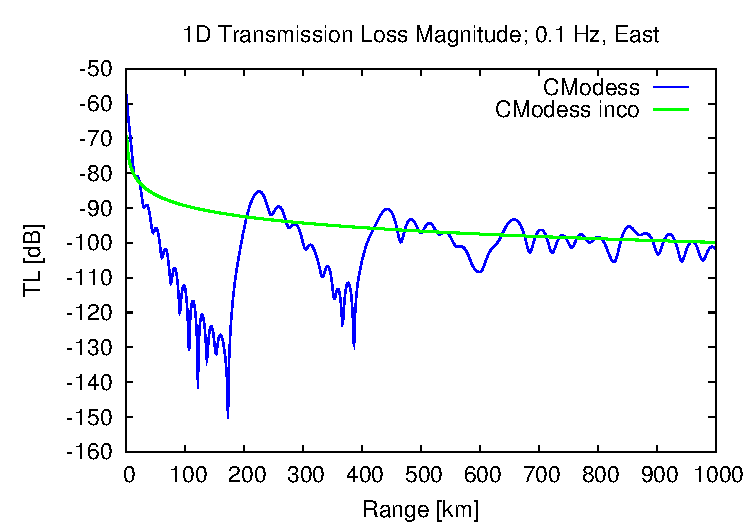
\includegraphics[scale=0.45]{figs/cmodess_ex1} 
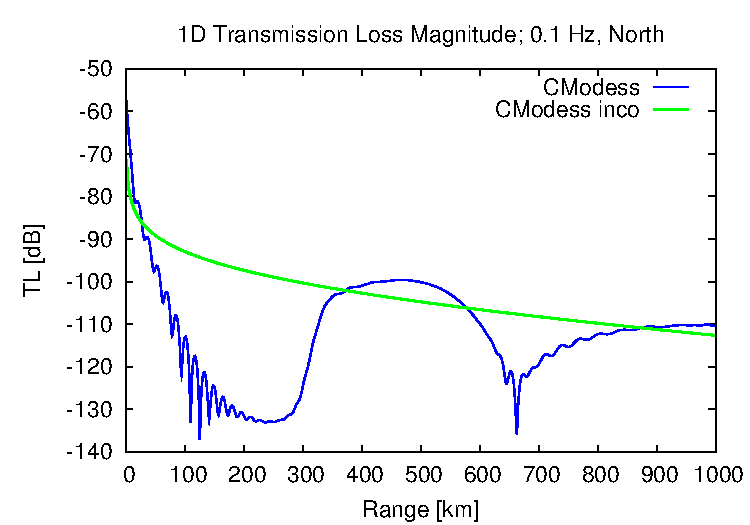
\includegraphics[scale=0.45]{figs/1D_cmodess_ex_N} 
\end{center}
\caption{1D transmission loss magnitude at 0.1 Hz obtained with {\bf CModess} for ground-to-ground propagation in the NCPA toy atmosphere shown in Figure \ref{fig:canonic_sound_speeds} for eastward, left plot, and northward, right plot. Shown are the transmission loss magnitude and incoherent transmission loss.}
\label{fig: cmodess 1D tl}
\end{figure}

The output is, by default, the one-dimensional (1D) transmission loss on the ground for both lossy and lossless cases and is written into the text files \verb+tloss_1d.cnm+ and \verb+tloss_1d.lossless.cnm+ as described above in the \verb+CModess+ help page; see section~\ref{sec:running cmodess} and section~\ref{sec:running modess} for more discussion. Examples of the magnitude of the complex 1D transmission loss output are shown in Figure \ref{fig: cmodess 1D tl}. Eastward propagation, as specified in the example above, and northward propagation, obtained by replacing \verb+--azimuth 90+ with  \verb+--azimuth 0+, are shown. Note that in general the output from all programs will be saved in the directory from which the code is run.  

In the second example the \verb+--write_2D_Tloss+ flag is appended to the command line entry for the first example: 
\begin{verbatim} 
    ../bin/CModess --atmosfile NCPA_canonical_profile_zuvwtdp.dat \ 
                   --atmosfileorder zuvwtdp --skiplines 0 --azimuth 90 \
                   --freq 0.1 --write_2D_TLoss
\end{verbatim}
As described above and in section~\ref{sec:running modess}, the output is written to a default file, in this case \verb+tloss2d.cnm+. The 2D transmission loss magnitude that results from eastward propagation, as specified in the example above, as well as northward propagation, obtained by replacing \verb+--azimuth 90+ with  \verb+--azimuth 0+, in the NCPA toy model is plotted in Figure \ref{fig: cmodess 2D tl}. 

\begin{figure}
\begin{center}
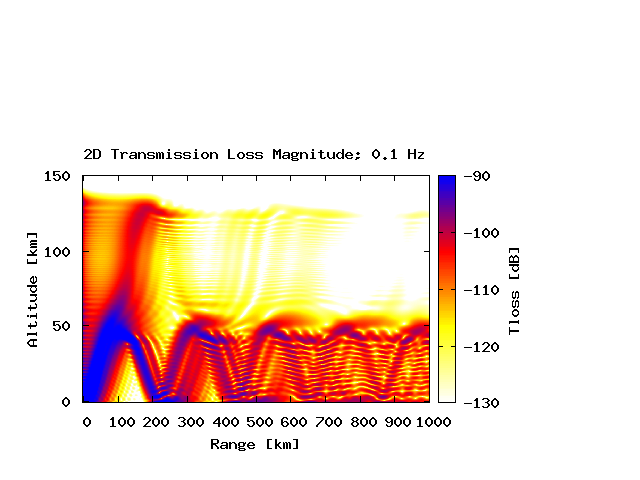
\includegraphics[scale=0.45,trim = 20 20 110 140,clip]{figs/cmodess_ex2}
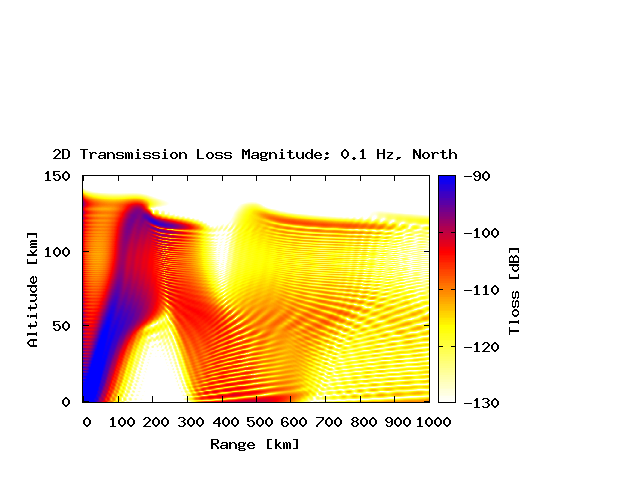
\includegraphics[scale=0.45,trim = 20 20 110 140,clip]{figs/2D_cmodess_ex_N}
\end{center}
\caption{2D transmission loss magnitude at 0.1 Hz obtained with {\bf CModess} for propagation from a source on the ground in the NCPA toy atmosphere shown in Figure \ref{fig:canonic_sound_speeds} for eastward, upper plot, and northward, lower plot, propagation.}
\label{fig: cmodess 2D tl}
\end{figure}

In the third example the \verb+--Nby2Dprop+ flag is appended to the command line entry for the first example. This flag requires that values for the options \verb+--azimuth_start+, \verb+--azimuth_end+, and \verb+--azimuth_step+ be given. 
\begin{verbatim} 
    ../bin/CModess --atmosfile NCPA_canonical_profile_zuvwtdp.dat \
                   --atmosfileorder zuvwtdp --skiplines 0 --freq 0.1 \
                   --Nby2Dprop --azimuth_start 0 --azimuth_end 360 --azimuth_step 1
\end{verbatim}
The output is written to the files \verb+Nby2D_tloss_1d.cnm+ and \verb+Nby2D_tloss_1d.lossless.cnm+ as described above in section~\ref{sec:running wmod}. The lossless transmission losses are also computed and saved as are the incoherent transmission losses. The resulting transmission loss magnitude is plotted in Figure \ref{fig: cmodess Nby2D tl}. 

\begin{figure}
\begin{center}
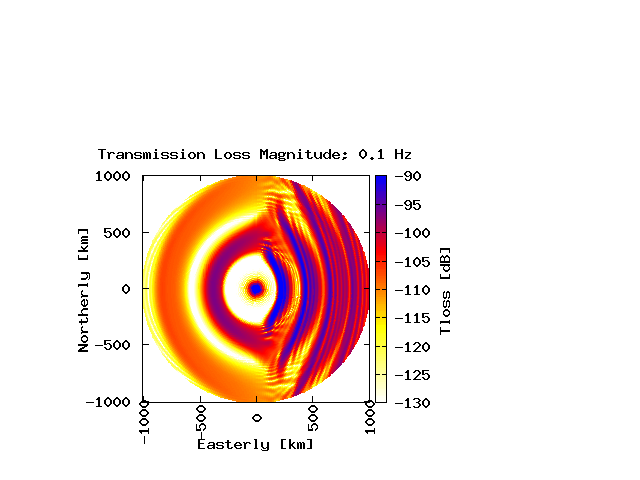
\includegraphics[scale=0.45,trim = 70 20 180 140,clip]{figs/cmodess_ex3}
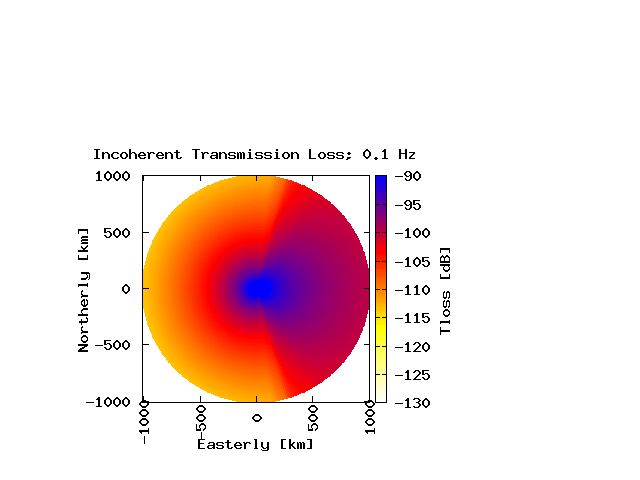
\includegraphics[scale=0.45,trim = 70 20 180 140,clip]{figs/cmodess_ex3_inco}
\end{center}
\caption{N by 2D transmission loss magnitude and incoherent transmission loss obtained with {\bf WMod} for ground-to-ground propagation in the NCPA toy model atmosphere from a source at the origin to all azimuths.}
\label{fig: cmodess Nby2D tl}
\end{figure}

In all these examples one will find that the runtimes are much longer than for \textbf{Modess}. The N by 2D run can take on the order of an hour, even at 0.1 Hz. It will take much longer at higher frequencies. 